% CREATED BY DAVID FRISK, 2016

% COVER PAGE
\begin{titlepage}
\newgeometry{top=3cm, bottom=3cm,
			left=2.25 cm, right=2.25cm}	% Temporarily change margins		
			
% Cover page background 
\AddToShipoutPicture*{\backgroundpic{-4}{56.7}{figure/auxiliary/frontpage_eng.pdf}}
\addtolength{\voffset}{2cm}

% Cover picture (replace with your own or delete)		
\begin{figure}[H]
\centering
\vspace{2cm}	% Adjust vertical spacing here
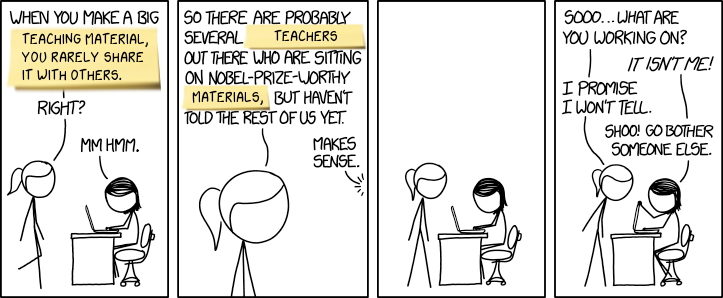
\includegraphics[width=\linewidth]{figure/xkcd.png}
\end{figure}

% Cover text
\mbox{}
\vfill
\renewcommand{\familydefault}{\sfdefault} \normalfont % Set cover page font
\textbf{{\Huge Accessibility of Teaching Materials 	}} 	\\[0.5cm]
{\Large Exploring Obtainability and Testing Usability \\[0.1cm] in Design of Shareable Teaching Materials}\\[0.5cm]
Master of Science thesis in Learning and Leadership \setlength{\parskip}{1cm}

{\Large HÅKAN ANDERSSON \\[0.2cm] SEBASTIAN EVERETT ERIKSSON} \setlength{\parskip}{2.9cm}

Department of Communication and Learning in Science \\
\textsc{Chalmers University of Technology} \\
Gothenburg, Sweden 2018

\renewcommand{\familydefault}{\rmdefault} \normalfont % Reset standard font
\end{titlepage}


% BACK OF COVER PAGE (BLANK PAGE)
\newpage
\restoregeometry
\thispagestyle{empty}
\mbox{}


% TITLE PAGE
\newpage
\thispagestyle{empty}
\begin{center}
	\textsc{\large Master's thesis 2018:NN}\\[4cm]		% Report number given by department 
	\textbf{\Large Accessibility of Teaching Materials} \\[1cm]
	{\large Exploring Obtainability and Testing Usability \\[0.1cm] in Design of Shareable Teaching Materials}\\[1cm]
	{\large HÅKAN ANDERSSON \\[0.1cm] SEBASTIAN EVERETT ERIKSSON}
	
	\vfill	
	% Logotype on titlepage	
	\begin{figure}[H]
	\centering
	% Remove the following line to remove the titlepage logotype
	
\includegraphics[width=0.2\pdfpagewidth]{figure/auxiliary/logo_eng.pdf} \\	
	\end{figure}	\vspace{5mm}	
	
	Department of Communication and Learning in Science \\
	\textsc{Chalmers University of Technology} \\
	Gothenburg, Sweden 2018 \\
\end{center}


% IMPRINT PAGE (BACK OF TITLE PAGE)
\newpage
\thispagestyle{plain}
\vspace*{4.5cm}
Accessibility of Teaching Materials:\\
Exploring Obtainability and Testing Usability \\ in Design of Shareable Teaching Materials\\
HÅKAN ANDERSSON \& SEBASTIAN EVERETT ERIKSSON  \setlength{\parskip}{1cm}

\copyright ~ HÅKAN ANDERSSON \& SEBASTIAN EVERETT ERIKSSON, 2018. \setlength{\parskip}{1cm}

Supervisor: Mats Ander, Department of Industrial and Materials Science\\
Examiner: Samuel Bengmark, Department of Mathematical Sciences \setlength{\parskip}{1cm}

Master's Thesis 2018:NN\\	% Report number given by department 
Department of Communication and Learning in Science\\
Chalmers University of Technology\\
SE-412 96 Gothenburg\\
Telephone +46 31 772 1000 \setlength{\parskip}{0.5cm}

\vfill
% Caption for cover page figure if used, possibly with reference to further information in the report
Cover: The comic strip is an adapted version of the \textit{xkcd} webcomic strip called \textit{Unpublished Discoveries} and aims to illustrate a teacher's unwillingness to share teaching material. In this study it is suggested one should instead request feedback from others during the design process, as a means to improve the end result. \\
{\scriptsize The original webcomic strip created by Randall Munroe can be found at \url{https://xkcd.com/1805/}, licensed under Creative Commons BY-NC 2.5. The font used for changing the original text is called \textit{xkcd script} and can be found at \url{https://github.com/ipython/xkcd-font}. It was provided under a Creative Commons BY-NC 3.0 license by the user \textit{ipython} on \textit{Github}. Licenses can be found at \url{https://creativecommons.org/licenses/by-nc/2.5/} and \url{https://creativecommons.org/licenses/by-nc/3.0/} respectively.} \setlength{\parskip}{0.5cm}

Typeset in \LaTeX \\
%Printed by [Name of printing company]\\
Gothenburg, Sweden 2018

